\documentclass{article}

\usepackage{booktabs}
\usepackage{tabularx}
\usepackage{hyperref}
\usepackage{graphicx}
\usepackage{float}
\usepackage{array}
\usepackage{pdflscape}
\usepackage{longtable}

\hypersetup{
    colorlinks=true,       % false: boxed links; true: colored links
    linkcolor=red,          % color of internal links (change box color with linkbordercolor)
    citecolor=green,        % color of links to bibliography
    filecolor=magenta,      % color of file links
    urlcolor=cyan           % color of external links
}

\title{Hazard Analysis\\\progname}

\author{\authname}

\date{}

\input{../Comments}
%% Common Parts

\newcommand{\progname}{Software Engineering} % PUT YOUR PROGRAM NAME HERE
\newcommand{\authname}{Team \#2, Team Name
\\ Zihao Du 
\\ Matthew Miller
\\ Firas Elayan
\\ Abhiram Neelamraju
\\ Michael Kim} % AUTHOR NAMES                  

\usepackage{hyperref}
    \hypersetup{colorlinks=true, linkcolor=blue, citecolor=blue, filecolor=blue,
                urlcolor=blue, unicode=false}
    \urlstyle{same}
                                


\begin{document}

\maketitle
\thispagestyle{empty}

~\newpage

\pagenumbering{roman}

\begin{table}[hp]
\caption{Revision History} \label{TblRevisionHistory}
\begin{tabularx}{\textwidth}{llX}
\toprule
\textbf{Date} & \textbf{Developer(s)} & \textbf{Change}\\
\midrule
Oct 20th & All & Revision 0\\
Nov 23rd & Zihao Du & Add the new requirement IDs in the new SRS\\
... & ... & ...\\
\bottomrule
\end{tabularx}
\end{table}

~\newpage

\tableofcontents

~\newpage

\pagenumbering{arabic}

\section{Introduction}

Based on the STPA Handbook, a system hazard is a system state or set of conditions that, together with a particular set of worst-case environmental conditions will lead to a loss. Regarding CampusConnections, our AR-based social networking application, a hazard can be a condition in the game when it fails to perform the intended functions or performs unexpected behaviors when coupled with environmental conditions. This document aims to detect, analyze, assess, and eliminate or migrate potential safety and security hazards that are applicable to this application. 

\section{Scope and Purpose of Hazard Analysis}

The scope of hazard analysis is to specify all potential system hazards that may arise when using the application and discover safety and security requirements to migrate and eliminate the effects of those hazards. However, it will not include hazards related to the hardware the application is running on. It will be the choice of the user and we cannot account for all mobile devices on the market. Hazard to the user and the society will be out of the scope as well. We will assume users intend to run the application on a normally functioning mobile device properly and efficiently. The purpose of the document is to highlight various hazards associated with the system, effects and causes of corresponding failures along with new requirements for further mitigation steps.

\section{System Boundaries and Components}
The system will be divided into the following components:
\begin{enumerate}
	\item The application's in-game feature components:
	      \begin{itemize}
		      \item Social Media
		      \item AR \& Location Services
		      \item Event/Lecture Management
		      \item General application features
	      \end{itemize}
	\item The database being used which will store all of users' data
	
\quad General app features include user login system, it will be responsible for user login and account creation, as well as notification and user accessibility management. The other three features are just responsible for corresponding in-game functionalities, more details can be found in the figure below. The database and user interaction are considered external to the system, the interaction between the system and external systems is described in the previous \href{https://github.com/beatlepie/4G06CapstoneProjectTeam2/blob/docs-hazard-analysis/docs/SRS-Volere/SRS.pdf}{document}.
\end{enumerate}
\begin{figure}[H]
\begin{center}
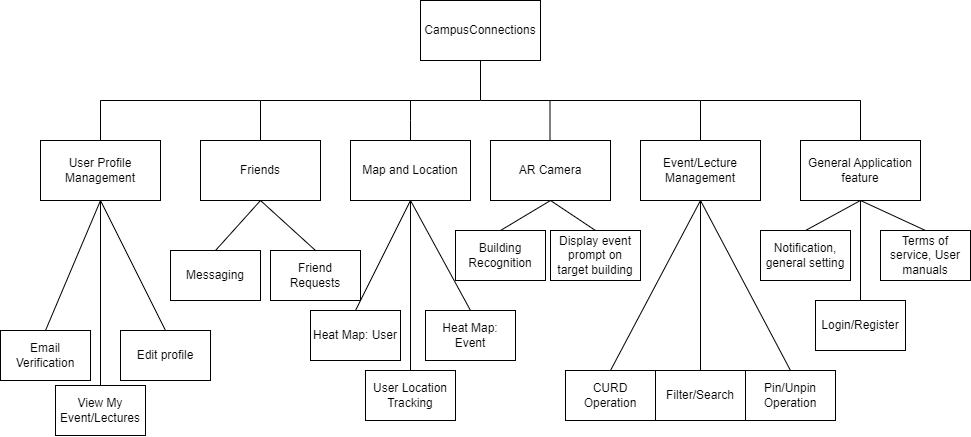
\includegraphics[scale=0.7]{components.png}
\end{center}
\caption{System Components}
\end{figure}
\section{Critical Assumptions}

\begin{itemize}
    \item Assume the users of the application do not intend to misuse it
    \item Assume the user's device will have all necessary hardware components with sufficient computing/output power such as sensors, processors, etc.
    \item Assume the routes to the backend of the system will always be ready to serve requests and not blocked due to unnecessarily locked resources
\end{itemize}

\section{Failure Mode and Effect Analysis}

\begin{landscape}
    \begin{longtable}{|>{\hspace{0pt}}m{0.075\linewidth}|>{\hspace{0pt}}m{0.102\linewidth}|>{\hspace{0pt}}m{0.106\linewidth}|>{\hspace{0pt}}m{0.156\linewidth}|>{\hspace{0pt}}m{0.169\linewidth}|>{\hspace{0pt}}m{0.242\linewidth}|>{\hspace{0pt}}m{0.033\linewidth}|>{\hspace{0pt}}m{0.044\linewidth}|} 
    \hline
    \multicolumn{1}{|>{\centering\hspace{0pt}}m{0.075\linewidth}|}{Design Function} & \multicolumn{1}{>{\centering\hspace{0pt}}m{0.102\linewidth}|}{Failure Modes} & \multicolumn{1}{>{\centering\hspace{0pt}}m{0.106\linewidth}|}{Causes of Failure} & \multicolumn{1}{>{\centering\hspace{0pt}}m{0.156\linewidth}|}{Effects of Failure} & \multicolumn{1}{>{\centering\hspace{0pt}}m{0.169\linewidth}|}{Detection} & \multicolumn{1}{>{\centering\hspace{0pt}}m{0.242\linewidth}|}{Recommended Action} & \multicolumn{1}{>{\centering\hspace{0pt}}m{0.033\linewidth}|}{SR} & \multicolumn{1}{>{\centering\arraybackslash\hspace{0pt}}m{0.044\linewidth}|}{Ref. No.} \endfirsthead 
    \hline
    AR Object Recognition & App is unable to detect object & Poor lighting conditions\par{}Camera angle & User is unable to view information from the AR element & Keep track of prior incomplete scan attempts & Implement a failsafe mechanism that shows the scannable information if enough previous attempts have failed & RFT2 AVR1 & H1 \\ 
    \hline
    Backend Server & Server is inaccessible & No internet connection\par{}Hosting service is down\par{}Invalid access key & Users are unable to make changes to their profile\par{}Users cannot receive updated information from the server & Keep track of the connection to the server using periodic heartbeats or similar methods & Display an error message stating that the connection the the server has been lost & RFT1 & H2 \\ 
    \hline
    User Profile View & Sensitive user data is publicly visible & Invalid visibility permissions\par{}Access control software malfunction & Confidential user information could be exposed and used for malicious purposes & Software failsafes and checks that verify the integrity of the permission structure & Prevent other users from accessing unauthorized information by creating a robust permissions system & SR & H3 \\ 
    \hline
    App Performance & App performance is poor & Large amounts of assets to be rendered\par{}Slow internet connection\par{}App is running on an old phone & User experiences lag or slowdown\par{}App feels unresponsive & Track of frame times or other performance metrics & Only show up to a maximum number of avatars or lower the level of detail & SLR & H4 \\ 
    \hline
    User Safety & App is used where and when it is not intended & User is distracted by the app & User could get into an accident & N/A & Display a warning message when opening the app that tells the user to be aware of their surroundings at all times while using the app & RFT2 & H5 \\ 
    \hline
    AR Module & Device is not compatible with AR features & Device is missing required hardware or software & User cannot use the AR features & Check if device supports the required feature set using API functions. & Display a warning message if the user's device is not compatible & RFT3 & H6 \\
    \hline
        Account Creation & Duplicate ID Creation &
            1.~ Account login failure
            2.~ Function returns incorrect results
            3.~ Incorrect user added as friend & 
            1.~ Duplicate ID was used during account creation 
            2.~ Duplicate ID was used during account update &
            Compare ID with existing ID in database & Checks whether the ID is duplicate or not when entered and when saving & IR & H7 \\
        \hline
        F7: Share location with friends & Location shown unintentionally &
            1.~ Location known without application being focused
            2.~ Incorrect location display on other users & 
            1.~ User did not turn off their GPS and application &
            Application only sends location information for too long & If user has not interacted with the application for a prolonged period, check for activity, and turn off all processes if no response is received & PR SR1 & H8 \\
        \hline
        Unauthorized user activity & 1.~ Incorrect login attempts 2.~ Account activity in unknown devices 3.~ Unknown administrator activity & 
            1.~ Account locked for user until further checks 
            2.~ Compromise of user and friend data & 
            1.~ Predictable passwords allowed, improper password change rules 
            2.~ Security measures such as second factor authentication not used
            3.~ Account lock features were not used & 
            1.~ Accounted used from previously unknown account
            2.~ Suspicious activity in the logs & 
            1.~ Too many incorrect passwords will result in account lock. The lock can be undone from email. The account ID and password can be changed with rules preventing predictable passwords such as cannot use same password.
            2.~ Recommend all users to use multi-factor authentication and have logs of their previous activity available to them.
            3. Notify users of the security measures of the application and procedures of using them & AR & H9 \\
         \hline
        Maintenance and updates of features & Update cannot be finished in time or major error is found & 
            1.~ Users could experience unexpected down times 2.~ Features could be delayed & 
            1.~ Update was not properly tested 
             & Maintenance expected time exceeds allocated time & Rollback to previous update and do the update sequencially in smaller patches at low usage times & MR & H10 \\    
\hline
    \end{longtable}
\end{landscape}

\section{Safety and Security Requirements}

The following requirements includes previous non-functional requirements in the Software Requirements Specification document that are referred in the previous section and new requirements added to handle potential hazards.

\subsection{Access Requirements}

There will be three levels of access. 

The first will be before login and account creation, where anyone can access. They must not have access to anything beyond the login, account creation, and account recovery pages.

The second will be after login that verifies their identity, where the user has provided information matching the McMaster student or faculty member with McMaster email account. Only the user can access this page.

The third level will the the administrator account, used for adding, deleting, or editing official events. This account can be accessed by login that verifies that they are the maintainer, this will be used by the maintainers to check the functionality of the product  and pull logs that are not accessible to users.

\subsection{Integrity Requirements}

The product will prevent introduction of duplicate data, to guarantee that all user identities are unique.

In the future, the database and server can protect itself from excessive use with a load balancer and additional servers being added.

\subsection{Privacy Requirements}

All data collected must be encrypted on disk in the server by standard encryption algorithm.
All data collected must be encrypted on transit by industry standard encryption algorithm.

The product will require users to agree on the terms prior to account creation and additional data submission.
The product must erase all data if the user requests, or when account is deleted.
Additionally, accounts that are inactive for a certain period of time will have their account deleted after notice to prevent unnecessary data being held.

\subsection{Audit Requirements}

N/A (This currently does not apply, once the product is ready to be used in multiple universities and regions, audit requirements will be reconsidered.)

\subsection{Immunity Requirements}

The product must only use open source libraries with many users and continuous security updates. 
As open source libraries are used by millions of people, vulnerabilities are found and patched much earlier.

The product must undergo vulnerability checks before a build is pushed to the users.
This will prevent vulnerabilities from inadequate codes from being introduced to user devices.

Security updates must be done as soon as possible when they are announced for used packages.
This will reduce the chances of novel attacks from affecting the product.

\subsection{New Requirements}
The new requirements are given new IDs in the revised SRS. Please check the following requirements in SRS for traceability purpose.\\
\textbf{PR1: P-SC4,\\ AVR1: P-RF6,\\ RTF1: P-RF3,\\ RFT2: P-RF4,\\ RTF3: P-RF5}.\\
\begin{itemize}
        \item[PR1.] \textbf{The product shall not transmit information while not in use.}
    \begin{itemize}
        \item \textbf{Rationale:} This requirement prevents the application from unnecessarily communicating with the server and taking up resources. This will improve the privacy and data protection of the application. This also reduces the battery usage of the product.
        \item \textbf{Fit Criterion:} The product will not execute any code that involves the transmission of information outside of the product.
    \end{itemize}
    \item[AVR1.] \textbf{There must be a failsafe for the product to function if server or internet connection takes too long or fails.}
    \begin{itemize}
        \item \textbf{Rationale:} This will allow the product to function to some degree even during high traffic or bad internet connection situations.
        \item \textbf{Fit Criterion:} The product must be able to provide rudimentary functionalities using its offline components.
    \end{itemize}
    \item[RFT1.] \textbf{The product shall display an error message when there is no internet connection.}
    \begin{itemize}
        \item \textbf{Rationale:} When there is no internet connection, the user should be made aware.
        \item \textbf{Fit Criterion:} An error message stating that there is no internet connection is displayed when the product fails to connect to the internet.
    \end{itemize}
    \item[RFT2.] \textbf{The product shall display a message upon startup warning the user to be aware of their surroundings.}
    \begin{itemize}
        \item \textbf{Rationale:} Ensures the safety of the user.
        \item \textbf{Fit Criterion:} A message telling the user to be aware of their surroundings is displayed upon startup.
    \end{itemize}
    \item[RFT3.] \textbf{The product shall display a warning message if the user's device is not compatible with the AR features.}
    \begin{itemize}
        \item \textbf{Rationale:} Tells the user that the AR features of the app cannot be used with their device.
        \item \textbf{Fit Criterion:} A warning message is displayed if the user's device is incompatible with AR.
    \end{itemize}
\end{itemize}

\section{Roadmap}

Safety Requirements to be implemented for capstone:
\begin{itemize}
    \item The product shall not transmit information while not in use.
    \item The product shall display an error message when there is no internet connection.
    \item The product shall display a message upon startup warning the user to be aware of their surroundings.
    \item The product shall display a warning message if the user's device is not compatible with the AR features.
\end{itemize}

\noindent
Safety Requirements to be implemented after capstone:
\begin{itemize}
    \item None
\end{itemize}

\end{document}